\documentclass[titlepage,a4paper]{article}

\usepackage{a4wide}
\usepackage[colorlinks=true,linkcolor=black,urlcolor=blue,bookmarksopen=true]{hyperref}
\usepackage{bookmark}
\usepackage{fancyhdr}
\usepackage{fancyvrb,newverbs,xcolor} % Para lcverbatim
\usepackage[spanish]{babel}
\usepackage[utf8]{inputenc}
\usepackage[T1]{fontenc}
\usepackage{graphicx}
\usepackage{hyperref}
\usepackage{float}
\usepackage[most]{tcolorbox}
\usepackage{longtable}

\pagestyle{fancy} % Encabezado y pie de página
\fancyhf{}
\fancyhead[L]{TdA1/TP1/106713/v1 - 106~713}
\fancyhead[R]{Teoría de Algoritmos I - FIUBA}
\renewcommand{\headrulewidth}{0.4pt}
\fancyfoot[C]{\thepage}
\renewcommand{\footrulewidth}{0.4pt}

% lcverbatim = Cuadro de código con fondo gris
\definecolor{cverbbg}{gray}{0.93}
\newenvironment{lcverbatim}
 {\SaveVerbatim{cverb}}
 {\endSaveVerbatim
  \flushleft\fboxrule=0pt\fboxsep=.5em
  \colorbox{cverbbg}{%
    \makebox[\dimexpr\linewidth-2\fboxsep][l]{\BUseVerbatim{cverb}}%
  }
  \endflushleft
}

\begin{document}
\begin{titlepage} % Carátula
	\hfill
\includegraphics[width=6cm]{logofiuba.jpg}
    \centering
    \vfill
    \Huge \textbf{Trabajo Práctico 1 — Karatsuba}
    \vskip2cm
    \Large [7529/9506] Teoría de Algoritmos I\\
    Segundo cuatrimestre de 2021
    \vfill
    \begin{tabular}{ | l | l | } % Datos del alumno
      \hline
      Alumno: & XXXXX~XXXXX, Xxxx \\ \hline
      Número de padrón: & 106~713 \\ \hline
      Email: & XXXXXX@fi.uba.ar \\ \hline
      Entrega: & nº 1 (29/09/2021) \\ \hline
  	\end{tabular}
    \vfill
    \vfill
\end{titlepage}

\tableofcontents % Índice general
\newpage

\section{Introducción}\label{sec:intro}
\subsection{Resumen}
El presente informe documenta el enunciado y la solución del primer trabajo práctico de la materia Teoría de Algoritmos I. El mismo comprende la resolución manual de una multiplicación mediante el algoritmo de Karatsuba junto con su análisis, así como una parte teórica sobre recursividad y Teorema Maestro.

Si bien este trabajo es individual, es redactado empleando el \href{http://aplica.rae.es/grweb/cgi-bin/v.cgi?i=OnqaThAvcEUygoXO}{plural de modestia} (tan usual en el ámbito académico).

\subsection{Lineamientos básicos}
\begin{itemize}
\item El trabajo se realizará en forma individual.

\item Se debe entregar el informe en formato pdf en el aula virtual de la materia.

\item El informe debe presentar carátula con datos del autor y fecha de entrega. Debe incluir número de hoja en cada página.

\item En caso de re-entrega, entregar un apartado con las correcciones mencionadas
\end{itemize}

\newpage\section{Parte 1: ¡Karatsuba!}\label{sec:parte1}

\subsection{Enunciado}

Dados los siguientes números (completada por su número de padrón):

\begin{lcverbatim}
    a35b411c
    2d98ef55
\end{lcverbatim}

con:

\begin{lcverbatim}
    a: dígito del padrón correspondiente a la unidad
    b: dígito del padrón correspondiente a la centena
    c: los dos dígitos del padrón de la izquierda mod 7
    d: dígito del padrón correspondiente a la decena
    e: dígito del padrón correspondiente a la unidad de mil
    f: los dos dígitos del padrón de la derecha mod 9
\end{lcverbatim}

Ejemplo. Padrón: 95473

\begin{lcverbatim}
33544114
27985155
\end{lcverbatim}

\noindent Se pide:

\begin{enumerate}
\item Resuelva la multiplicación paso a paso utilizando el algoritmo de Karatsuba.

\item Cuente la cantidad de sumas y multiplicaciones que realiza y relaciónelo con la complejidad temporal del método.

\item Comparar lo obtenido con el método de multiplicación tradicional. ¿Observa alguna mejora? Analice.

\item ¿Por qué se puede considerar al algoritmo de Karatsuba como de “división y conquista”?
\end{enumerate}

\newpage\subsection{Resolución con Karatusba}
\begin{tcolorbox}[colback=blue!5!white,colframe=blue!75!black,title=Enunciado 1.1]
    Resuelva la multiplicación paso a paso utilizando el algoritmo de Karatsuba.
\end{tcolorbox}
\subsubsection{Adaptación de productos al número de padrón}
Comenzaremos realizando la adaptación del número según el padrón 106~713:
\begin{lcverbatim}
    a: dígito del padrón correspondiente a la unidad = 3
    b: dígito del padrón correspondiente a la centena = 7
    c: los dos dígitos del padrón de la izquierda mod 7 = 10 mod 7 = 3
    d: dígito del padrón correspondiente a la decena = 1
    e: dígito del padrón correspondiente a la unidad de mil = 6
    f: los dos dígitos del padrón de la derecha mod 9 = 13 mod 9 = 4
\end{lcverbatim}
Por lo que el resultado es:
\begin{lcverbatim}
    33574113 
    21986455
\end{lcverbatim}
\subsubsection{Detalles generales y  de la función recursiva}
También definimos que trabajaremos en base decimal, por lo que en cada etapa de recursión (hasta llegar a $n=1$):
\begin{itemize}
    \item convertiremos los productos $X$ e $Y$ en:
    $$X \rightarrow X_1\times 10^{n/10}+X_0$$
    $$Y \rightarrow Y_1\times 10^{n/10}+Y_0$$
    Es decir, sabiendo que $D = 10^{\lceil n/2\rceil}$:
    $$X_0 = X \mod D, \quad X_1 = \lfloor X / D \rfloor$$
    $$Y_0 = Y \mod D, \quad Y_1 = \lfloor Y / D \rfloor$$
    \item Calculamos\footnote{El uso de $P_X$, $P_Y$, $M_1$ y $M_2$ corresponde a una notación propia de este informe (para mayor claridad), no al material de estudio.} $P_X=X_0+X_1$ e $P_Y=Y_0+Y_1$.
    \item Obtendremos recursivamente (para n>1) las 3 multiplicaciones\footnotemark[\value{footnote}]:
    $$M_0 = X_0\times Y_0,\quad M_1 = X_1\times Y_1,\quad P = P_X\times P_Y$$
    \item Realizamos las sumas y desplazamientos (multiplicación por potencia de la base elegida: $10^k$):
    $$M_1\times 10^n + (P-M_1-M_0)\times 10^{n/2} + M_0$$
\end{itemize}

Una vez alcanzado el caso base, se obtendrá el resultado mediante una clásica tabla de multiplicar de 1 cifra decimal.

\subsubsection{Etapas de recursión del caso dado}
Para mantener la claridad de la explicación paso a paso, comenzaremos tan solo mostrando cuáles son las cuentas que deben realizarse en cada etapa de recursión.

\begin{figure}[H]
\centering
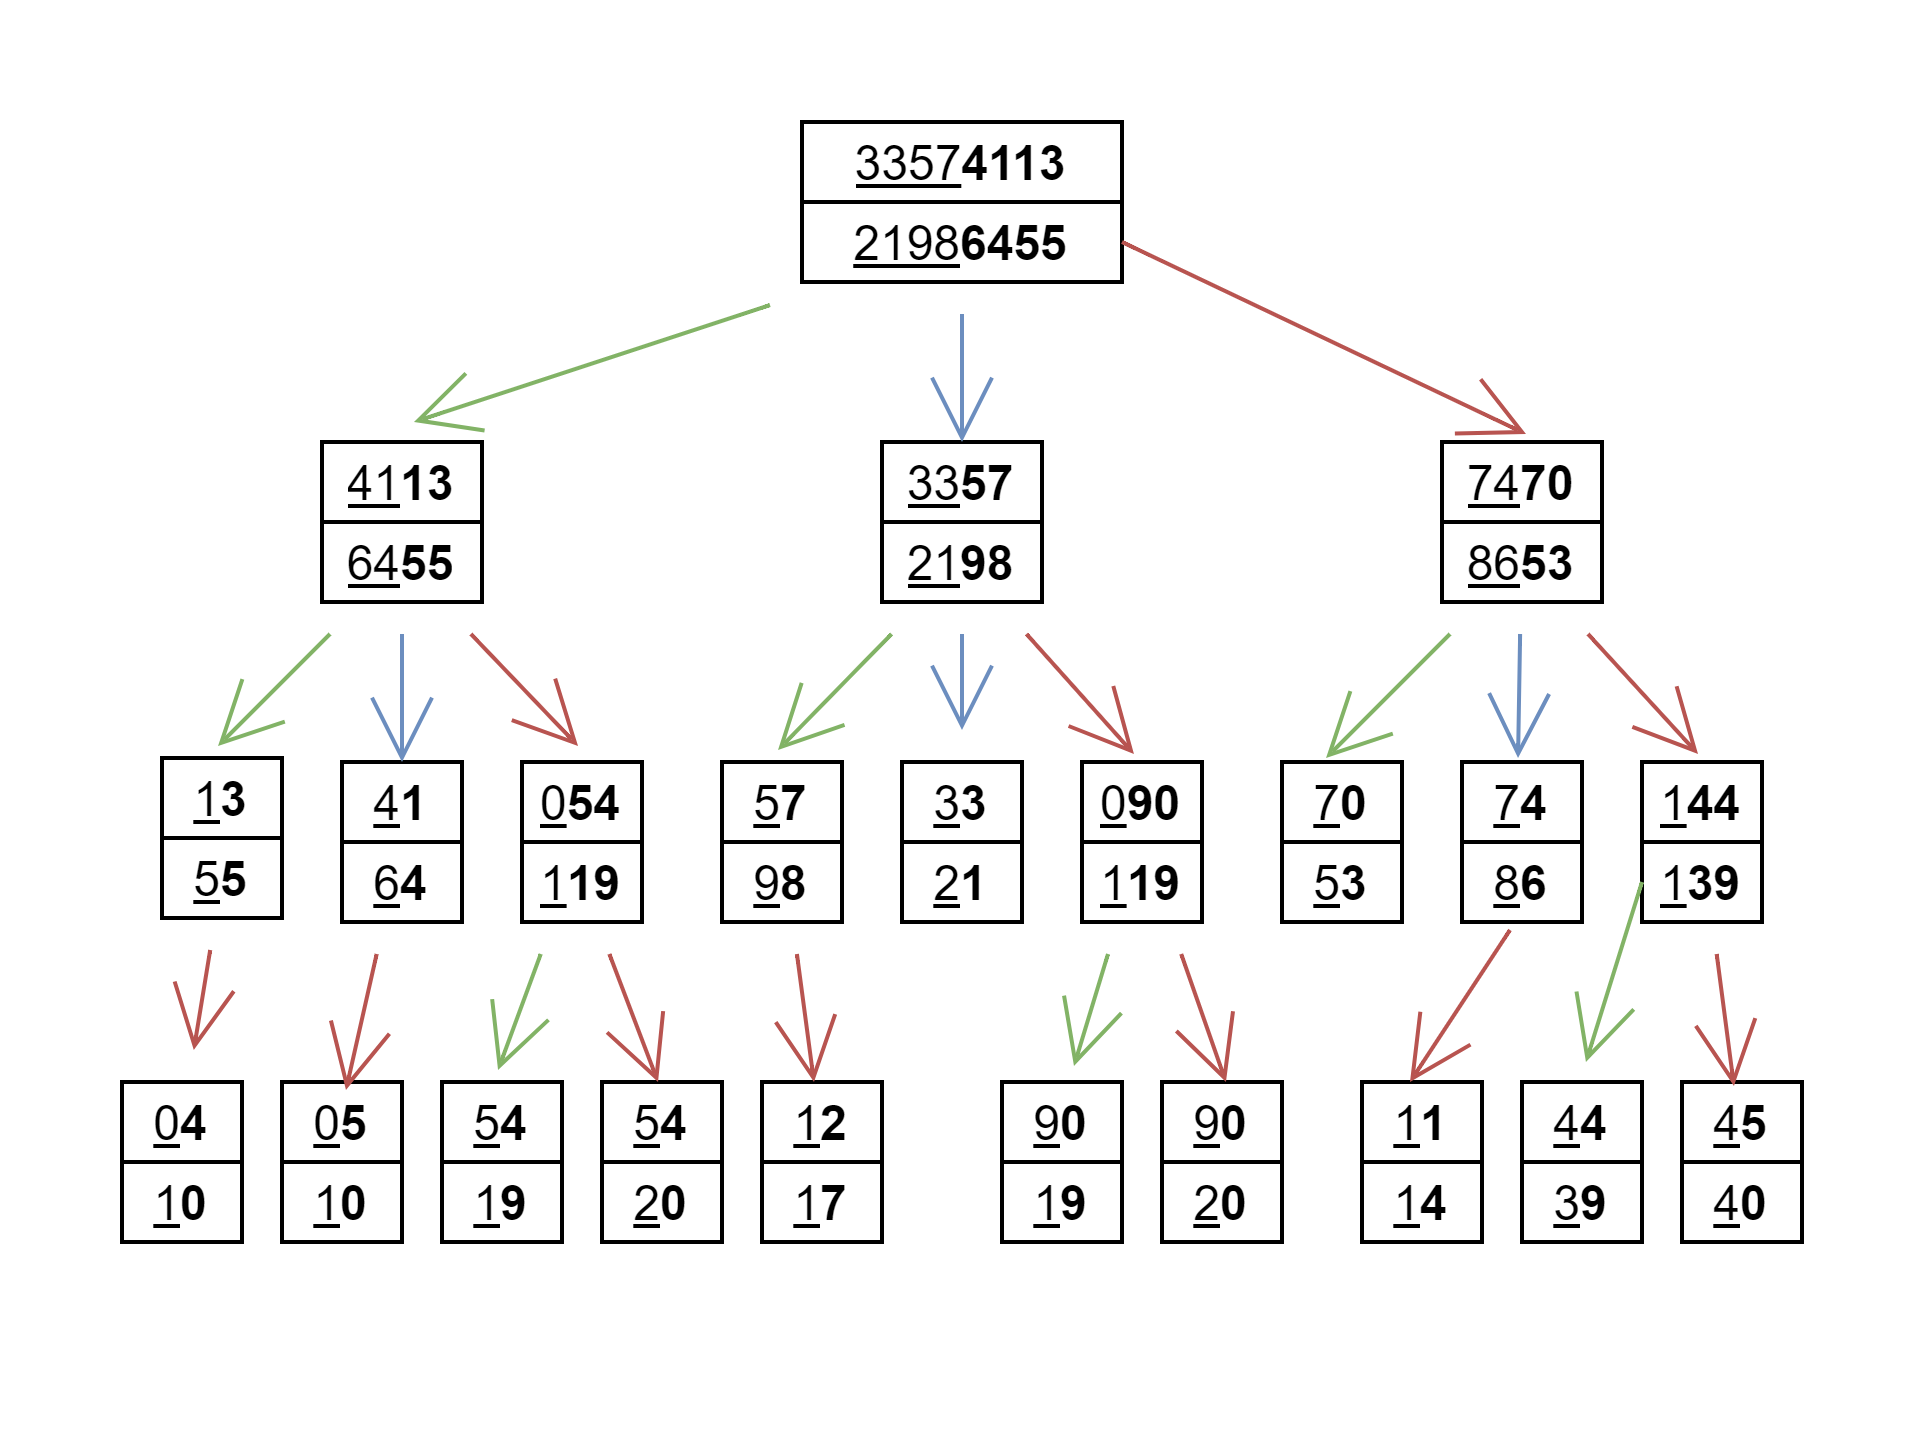
\includegraphics[width=\textwidth]{Karatsuba106713.drawio.png}
\caption{\label{fig:etapas}}\textbf{Etapas de recursión de Karatsuba} para el caso dado. Cada nodo consiste del X e Y de cada llamada a la función, pero los casos bases (n=1) han sido omitidos. La parte inferior ($X_0$ e $Y_0$) han sido remarcadas con subrayados, mientras que la superior ($X_1$ e $Y_1$) con negritas. En verde el cálculo de $M_0$ (producto de partes inferiores), en azul $M_1$ (de partes superiores) y en rojo $P$ (producto de suma de partes equivalentes de cada entrada).
\end{figure}
El siguiente listado incluye todas las llamadas a la función, y en el caso en que corresponda (cuando n>1) se detalla qué función llama cada una:
\begin{lcverbatim}
Etapa 1:
	Llamada 1.1: Karatsuba(33574113, 21986455). Req.:
		M0=karatsuba(4113,6455),M1=karatsuba(3357,2198),P=karatsuba(7470,8653).
\end{lcverbatim}
\begin{lcverbatim}
Etapa 2:
	Llamada 2.1: Karatsuba(4113, 6455). Req.:
		M0=karatsuba(13,55),M1=karatsuba(41,64),P=karatsuba(54,119).
	Llamada 2.2: Karatsuba(3357, 2198). Req.:
		M0=karatsuba(57,98),M1=karatsuba(33,21),P=karatsuba(90,119).
	Llamada 2.3: Karatsuba(7470, 8653). Req.:
		M0=karatsuba(70,53),M1=karatsuba(74,86),P=karatsuba(144,139).
\end{lcverbatim}
\begin{lcverbatim}
Etapa 3:
	Llamada 3.1: Karatsuba(13, 55). Req.:
		M0=karatsuba(3,5),M1=karatsuba(1,5),P=karatsuba(4,10).
	Llamada 3.2: Karatsuba(41, 64). Req.:
		M0=karatsuba(1,4),M1=karatsuba(4,6),P=karatsuba(5,10).
	Llamada 3.3: Karatsuba(54, 119). Req.:
		M0=karatsuba(54,19),M1=karatsuba(0,1),P=karatsuba(54,20).
	Llamada 3.4: Karatsuba(57, 98). Req.:
		M0=karatsuba(7,8),M1=karatsuba(5,9),P=karatsuba(12,17).
	Llamada 3.5: Karatsuba(33, 21). Req.:
		M0=karatsuba(3,1),M1=karatsuba(3,2),P=karatsuba(6,3).
	Llamada 3.6: Karatsuba(90, 119). Req.:
		M0=karatsuba(90,19),M1=karatsuba(0,1),P=karatsuba(90,20).
	Llamada 3.7: Karatsuba(70, 53). Req.:
		M0=karatsuba(0,3),M1=karatsuba(7,5),P=karatsuba(7,8).
	Llamada 3.8: Karatsuba(74, 86). Req.:
		M0=karatsuba(4,6),M1=karatsuba(7,8),P=karatsuba(11,14).
	Llamada 3.9: Karatsuba(144, 139). Req.:
		M0=karatsuba(44,39),M1=karatsuba(1,1),P=karatsuba(45,40).
\end{lcverbatim}
\begin{lcverbatim}
Etapa 4:
	Llamada 4.3: Karatsuba(4, 10). Req.:
		M0=karatsuba(4,0),M1=karatsuba(0,1),P=karatsuba(4,1).
	Llamada 4.6: Karatsuba(5, 10). Req.:
		M0=karatsuba(5,0),M1=karatsuba(0,1),P=karatsuba(5,1).
	Llamada 4.7: Karatsuba(54, 19). Req.:
		M0=karatsuba(4,9),M1=karatsuba(5,1),P=karatsuba(9,10).
	Llamada 4.9: Karatsuba(54, 20). Req.:
		M0=karatsuba(4,0),M1=karatsuba(5,2),P=karatsuba(9,2).
	Llamada 4.12: Karatsuba(12, 17). Req.:
		M0=karatsuba(2,7),M1=karatsuba(1,1),P=karatsuba(3,8).
	Llamada 4.16: Karatsuba(90, 19). Req.:
		M0=karatsuba(0,9),M1=karatsuba(9,1),P=karatsuba(9,10).
	Llamada 4.18: Karatsuba(90, 20). Req.:
		M0=karatsuba(0,0),M1=karatsuba(9,2),P=karatsuba(9,2).
	Llamada 4.24: Karatsuba(11, 14). Req.:
		M0=karatsuba(1,4),M1=karatsuba(1,1),P=karatsuba(2,5).
	Llamada 4.25: Karatsuba(44, 39). Req.:
		M0=karatsuba(4,9),M1=karatsuba(4,3),P=karatsuba(8,12).
	Llamada 4.27: Karatsuba(45, 40). Req.:
		M0=karatsuba(5,0),M1=karatsuba(4,4),P=karatsuba(9,4).
\end{lcverbatim}
\begin{lcverbatim}
Etapa 5:
	Llamada 5.9: Karatsuba(9, 10). Req.:
		M0=karatsuba(9,0),M1=karatsuba(0,1),P=karatsuba(9,1).
	Llamada 5.18: Karatsuba(9, 10). Req.:
		M0=karatsuba(9,0),M1=karatsuba(0,1),P=karatsuba(9,1).
	Llamada 5.27: Karatsuba(8, 12). Req.:
		M0=karatsuba(8,2),M1=karatsuba(0,1),P=karatsuba(8,3).
\end{lcverbatim}

\newpage\subsubsection{Resolución de cada etapas, paso a paso}

Ahora, conociendo los cálculos necesarios en cada etapa, comenzaremos a resolverlos desde la más profunda (los casos base, de $n=1$) hasta llegar a la más superficial (el problema planteado, de $n=8$).
\par
\vspace{3em}
\par
\begin{longtable}[r]{lllllll}
%\begin{table}[]
%\begin{tabular}{lllllll}

1.1: & \multicolumn{6}{l}{ $ Karatsuba(33574113, 21986455) n=8 \implies D = 10^{\lceil 8/2\rceil} = 10^4$ }\\
     & 1.1.1:     & \multicolumn{5}{l}{$X\_0 = 33574113 \mod 10^4 = 4113, \quad X\_1 = \lfloor 33574113 / 10^4 \rfloor = 3357$}     \\
     & 1.1.2:     & \multicolumn{5}{l}{$Y\_0 = 21986455 \mod 10^4 = 6455, \quad Y\_1 = \lfloor 21986455 / 10^4 \rfloor = 2198$}     \\
     & 1.1.3:     & \multicolumn{5}{l}{$P\_X = X\_0+X\_1 = 4113 + 3357 = 7470,\quad P\_Y = Y\_0+Y\_1 = 6455 + 2198 = 8653$}     \\
     & 1.1.4:     & \multicolumn{5}{l}{$M\_0=karatsuba(4113,6455)=$ … Llamada a 2.1 ($n=4 \implies D=10^{\lceil 4/2\rceil} = 10^2$}     \\

\multicolumn{2}{l}{}     & 2.1.1:     & \multicolumn{4}{l}{$X\_0=13, X\_1=41$}     \\
\multicolumn{2}{l}{}     & 2.1.2:     & \multicolumn{4}{l}{$Y\_0=55, Y\_1=64$}     \\
\multicolumn{2}{l}{}     & 2.1.3:     & \multicolumn{4}{l}{$P\_X=13+41=54, P\_Y=55+64=119$}     \\
\multicolumn{2}{l}{}     & 2.1.4:     & \multicolumn{4}{l}{$M0=karatsuba(13,55)$. Llamada a 3.1 ($n=2,D=10$)}     \\

\multicolumn{3}{l}{}     & 3.1.1:     & \multicolumn{3}{l}{}     \\
\multicolumn{3}{l}{}     & 3.1.2:     & \multicolumn{3}{l}{}     \\
\multicolumn{3}{l}{}     & 3.1.3:     & \multicolumn{3}{l}{}     \\
\multicolumn{3}{l}{}     & 3.1.4:     & \multicolumn{3}{l}{$M0=karatsuba(3,5) = 15$}     \\
\multicolumn{3}{l}{}     & 3.1.5:     & \multicolumn{3}{l}{$M1=karatsuba(1,5) = 5$}     \\
\multicolumn{3}{l}{}     & 3.1.6:     & \multicolumn{3}{l}{$P=karatsuba(4,10)$. Llamada 4.3 ($n=2, D=10$)}     \\

\multicolumn{4}{l}{}     & 4.3.1:     & \multicolumn{2}{l}{}     \\
\multicolumn{4}{l}{}     & 4.3.2:     & \multicolumn{2}{l}{}     \\
\multicolumn{4}{l}{}     & 4.3.3:     & \multicolumn{2}{l}{}     \\
\multicolumn{4}{l}{}     & 4.3.4:     & \multicolumn{2}{l}{$M0=karatsuba(4,0)=0$}     \\
\multicolumn{4}{l}{}     & 4.3.5:     & \multicolumn{2}{l}{$M1=karatsuba(0,1)=0$}     \\
\multicolumn{4}{l}{}     & 4.4.6:     & \multicolumn{2}{l}{$P=karatsuba(4,1)=4$}     \\
\multicolumn{4}{l}{}     & 4.3.7:     & \multicolumn{2}{l}{$\leftarrow 0\times 10^2 + (4-0-0)\times 10 = 0 + 40 + 0 = \boxed{40}$} \\

\multicolumn{3}{l}{}     & 3.1.7:     & \multicolumn{3}{l}{$\leftarrow 5\times 10^2 + (40 - 5 - 15)\times 10 + 15 = 500 + 200 + 15 = \boxed{715}$}

%\end{tabular}
%\end{table}
\end{longtable}

\begin{lcverbatim}
    A completar
\end{lcverbatim}

\subsection{Cantidad de operaciones y complejidad}

\begin{tcolorbox}[colback=blue!5!white,colframe=blue!75!black,title=Enunciado 1.2]
    Cuente la cantidad de sumas y multiplicaciones que realiza y relaciónelo con la complejidad temporal del método.
\end{tcolorbox}

\begin{lcverbatim}
    A completar
\end{lcverbatim}


\subsection{Comparación con algoritmo tradicional}
\begin{tcolorbox}[colback=blue!5!white,colframe=blue!75!black,title=Enunciado 1.3]
    Comparar lo obtenido con el método de multiplicación tradicional. ¿Observa alguna mejora? Analice.
\end{tcolorbox}

\begin{lcverbatim}
    A completar
\end{lcverbatim}


\subsection{División y conquista}

\begin{tcolorbox}[colback=blue!5!white,colframe=blue!75!black,title=Enunciado 1.4]
    ¿Por qué se puede considerar al algoritmo de Karatsuba como de “división y conquista”?
\end{tcolorbox}

Para que un algoritmo sea considerado de "divide y conquista" debe dividir sus datos de entrada, \textbf{llamarse recursivamente}, una o varias veces, \textbf{con una fracción de los datos} (hasta un caso base que resulte trivial o se resuelva mediante otro algoritmo) y finalmente unificar los resultados para formar una solución.

Es notable destacar que no es una condición necesaria que haya una relación unívoca entre las características de la división y la cantidad de llamadas. Así, pueden encontrarse algoritmos como la búsqueda binaria, en la que se fracciona en 2 partes iguales, pero sólo se invoca la recursión sobre una mitad. De manera análoga pero inversa, el algoritmo de Karatsuba realiza (excepto en el caso base) tres llamadas recursivas con datos de la mitad del tamaño de los de entrada.

En todo caso, sí son condiciones necesarias que en cada llamada recursiva la cantidad de datos disminuya \textbf{acercándose al caso base}, y que el algoritmo aplicado sea el mismo. \textbf{Por todo esto, podemos afirmar que el algoritmo de Karatsuba puede considerarse como un algoritmo de “división y conquista”}.





\newpage\section{Parte 2: Cuestión de complejidad…}\label{sec:parte2}

\subsection{Enunciado}

Dada la siguiente relación de recurrencia
\begin{lcverbatim}
    a T(n/b) + O(c)
\end{lcverbatim}

Con:

\begin{lcverbatim}
a: 1 + (los dos dígitos del padrón de la izquierda mod 9)
b: 2 + (los dos dígitos del padrón de la izquierda mod 7)
c: “n” si su padrón es múltiplo de 4, 
   sino “nlogn” si su padrón es múltiplo de 3,
   sino “n2”  \end{lcverbatim}
\noindent Se pide:
\begin{enumerate}
\item Responda y complete: ¿Qué le falta a la relación de recurrencia para que se pueda aplicar el teorema maestro?

\item Calcular la complejidad temporal utilizando el teorema maestro.

\item Explique paso a paso cómo llega a la misma.

\end{enumerate}

\newpage\subsection{Teorema maestro}
\begin{tcolorbox}[colback=blue!5!white,colframe=blue!75!black,title=Enunciado 2.1]
    Responda y complete: ¿Qué le falta a la relación de recurrencia para que se pueda aplicar el teorema maestro?
\end{tcolorbox}

\subsection{Complejidad temporal}
\begin{tcolorbox}[colback=blue!5!white,colframe=blue!75!black,title=Enunciado 2.2]
    Calcular la complejidad temporal utilizando el teorema maestro.
\end{tcolorbox}

\begin{tcolorbox}[colback=blue!5!white,colframe=blue!75!black,title=Enunciado 2.3]
    Explique paso a paso cómo llega a la misma.
\end{tcolorbox}

\begin{lcverbatim}
    A completar
\end{lcverbatim}

\end{document}
